% !TeX spellcheck = fr_FR
\documentclass[../main.tex]{subfiles}

\begin{document}

\subsection{Données synthétiques}\label{ssec:synthResults}

Les modèles ont été entraînés sur des jeux de données synthétiques générées à partir d'un processus de Hawkes linéaire à noyau exponentiel, en utilisant la librairie \verb|tick| pour Python \cite{2017arXiv170703003B}.

Un indicateur de performance pertinent est de regarder la distribution du nombre d'événements total $N_T$ ou par type d'événement $N^k_T, k\in\llbracket 1,K\rrbracket$.

On a utilisé deux jeux de données synthétiques.

Le premier jeu de données est un processus de Hawkes en dimension $K=1$ avec $\mu=1$, $\alpha = 0.5$, $\beta = 3.0$ et $T = 60$ (en secondes).

Le modèle Decay-RNN réussit à répliquer correctement le comportement d'un processus de Hawkes en dimension 1, comme l'illustrent la distribution de $N_T$ \autoref{fig:hawkes1DDecayRNNlengthDistrib} et le graphe de l'intensité \autoref{fig:hawkes1DRNNintensityPlot}.

\begin{figure}[htp]
	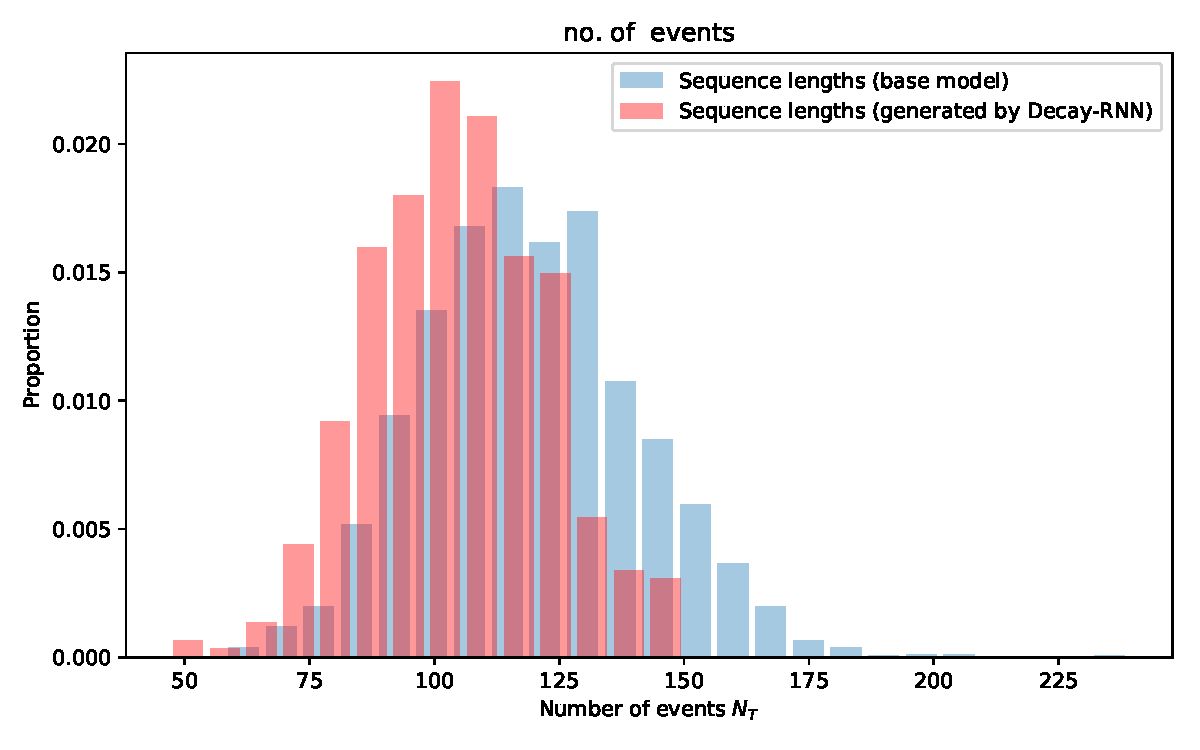
\includegraphics[width=\linewidth]{../results/seq_length_distrib_Decay-RNN-1d-hidden_6-20181201-220235.pdf}
	\caption{Distribution du nombre d'événements. $K=1$ type d'événements. Hawkes vs. Decay-RNN avec $D=6$ neurones cachés.}\label{fig:hawkes1DDecayRNNlengthDistrib}
\end{figure}

\begin{figure}[htp]
	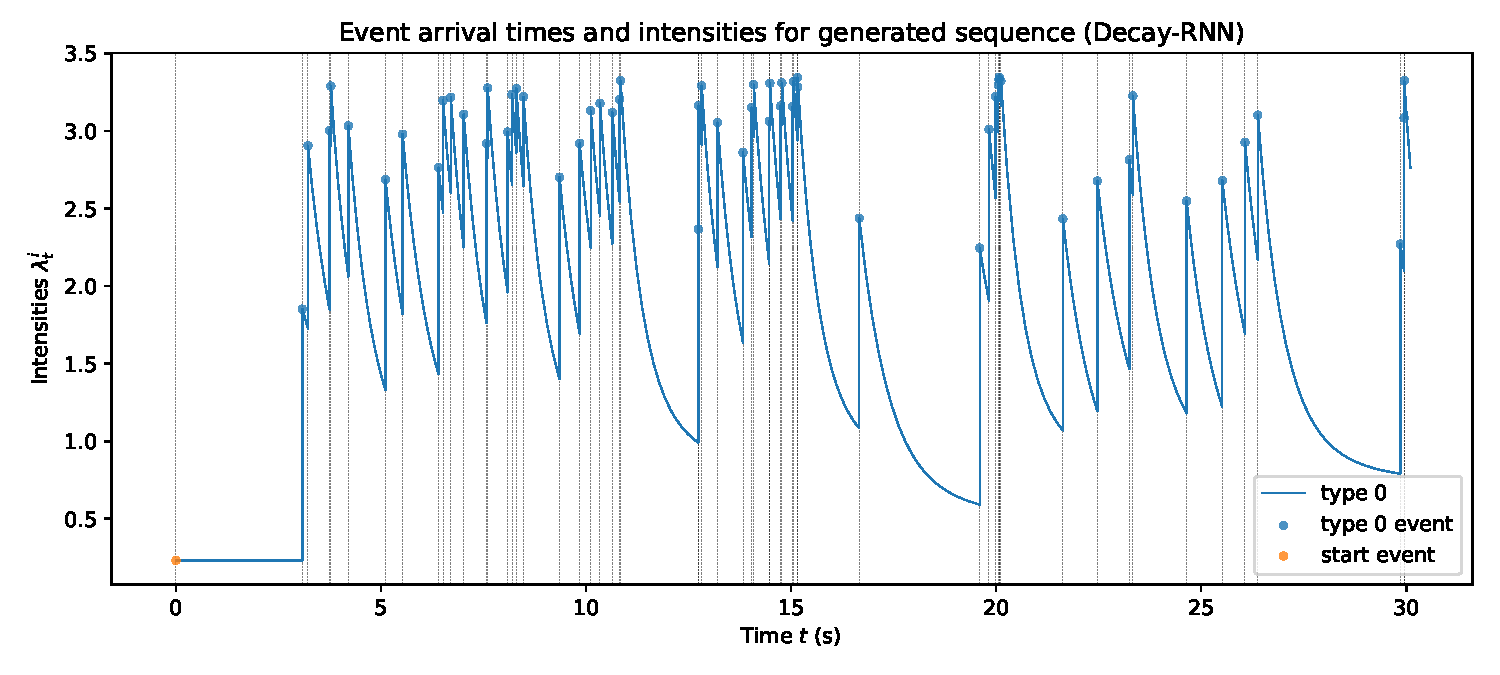
\includegraphics[width=\linewidth]{../results/intensity_Decay-RNN_1d_hidden6_20181201-220235.pdf}
	\caption{Processus d'intensité et temps d'arrivée, séquence générée par le modèle Decay-RNN après entraînement.}\label{fig:hawkes1DRNNintensityPlot}
\end{figure}

\begin{figure}[htp]
	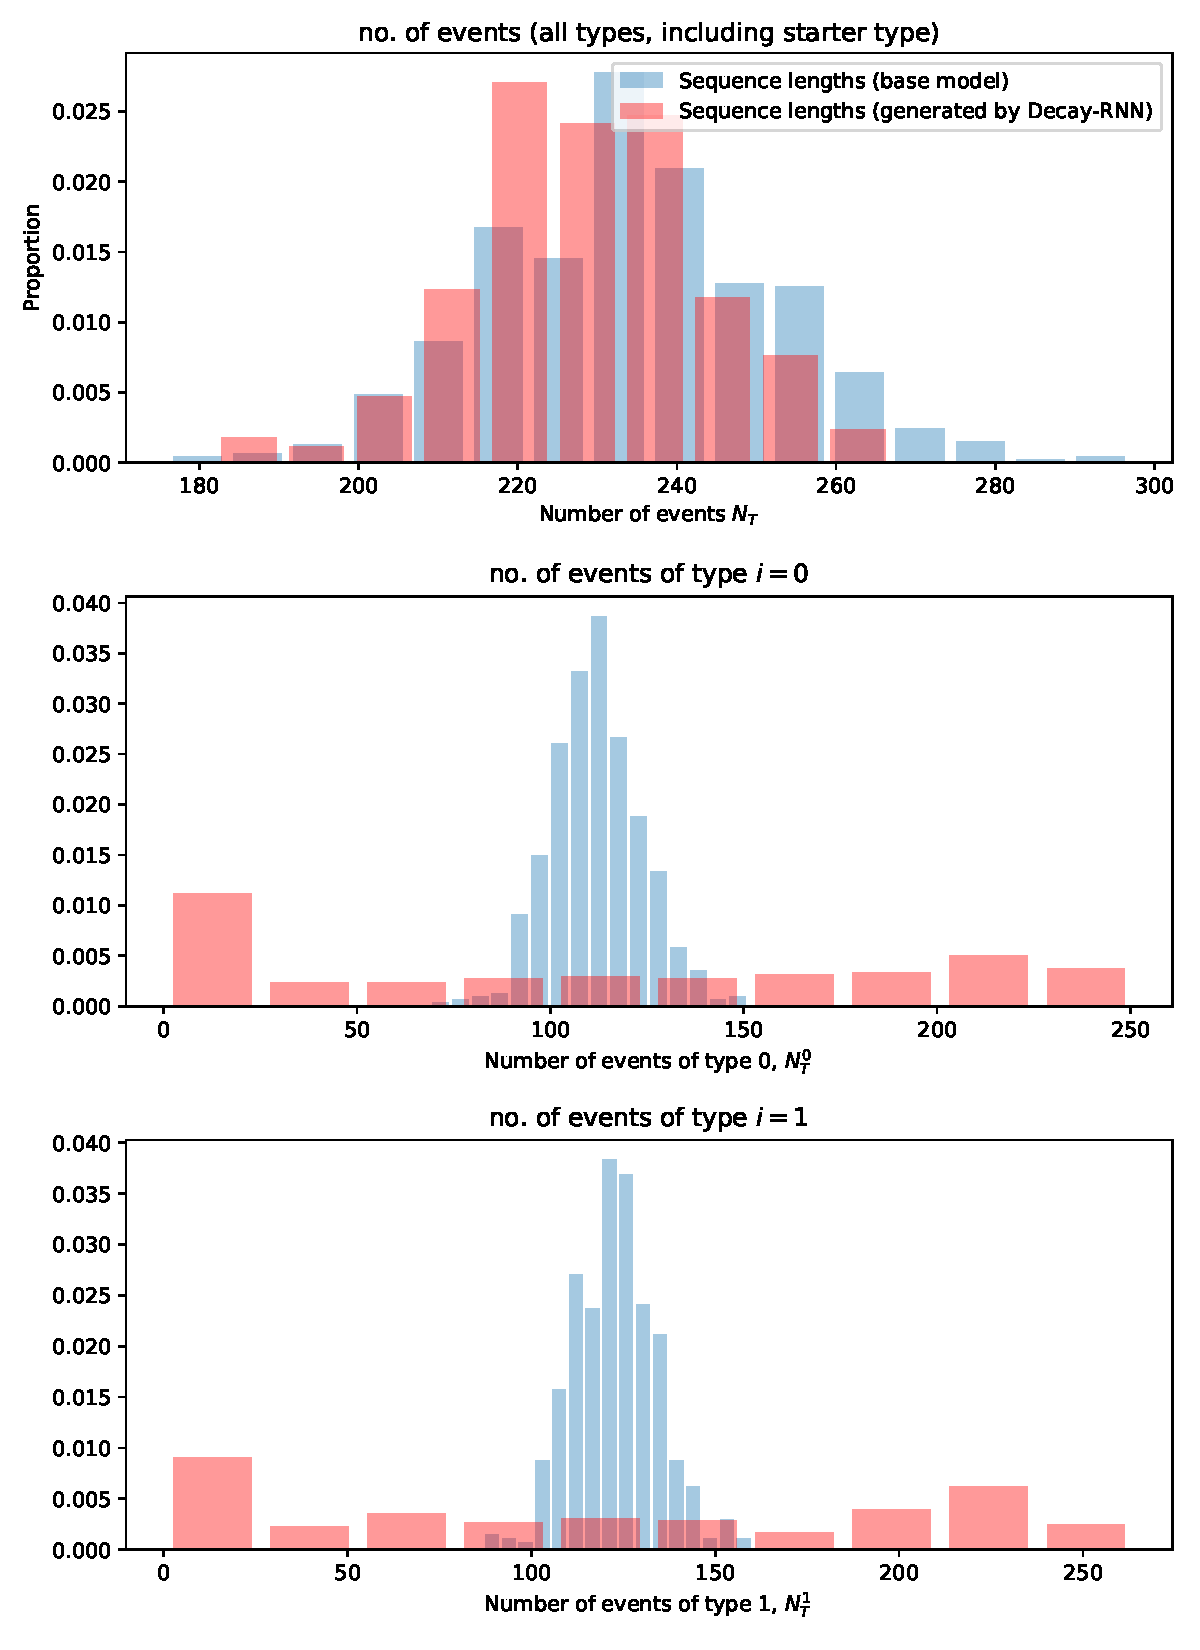
\includegraphics[width=\linewidth]{../results/seq_length_distrib_Decay-RNN-2d-hidden_12-20181201-003410.pdf}
	\caption{Distribution du nombre d'événements. Hawkes bidimensionnel vs. Decay-RNN avec $D=12$ neurones cachés.}\label{fig:hawkes2DDecayRNNlengthDistrib}
\end{figure}

\end{document}